\section{Component Types}
With the introduction of software components, the question of their substitutability and conformance arises. A component is not only defined by its provided interfaces, but also by the interfaces required from the environment. So, the constraints for replacing a component in its context are more complex than, for example, the constraints for replacing a class that implements a set of interfaces. The UML 2.0 superstructure addresses this issue only curtly:

\begin{quote}
``As such, a component serves as a type whose conformance is defined by these provided and required interfaces $[\ldots]$. One component may therefore be substituted by another only if the two are type conformant \cite[p.142]{OMGUML2005a}.''
%TODO add reference: UML Superstructure p.150
\end{quote}

Here, the terms \emph{component type} and \emph{conformance} of components and types are mentioned. However, both concepts are not further clarified. We need a clear definition of both terms to provide a component meta model that allows (a)  interoperability and substitutability checks of components and (b) enables the prediction of Quality of Service attributes of a component in a certain context.

In the following, we develop a more detailed approach to component types that allows different notions of substitutability. We also clarify the conformance of a component to a type. We introduce these concepts using the architecture of a web server shown in figure \ref{fig:WebserverComponents} and give a formal definition of the terms at the end of this section.

\begin{figure}[htbp]
\centering
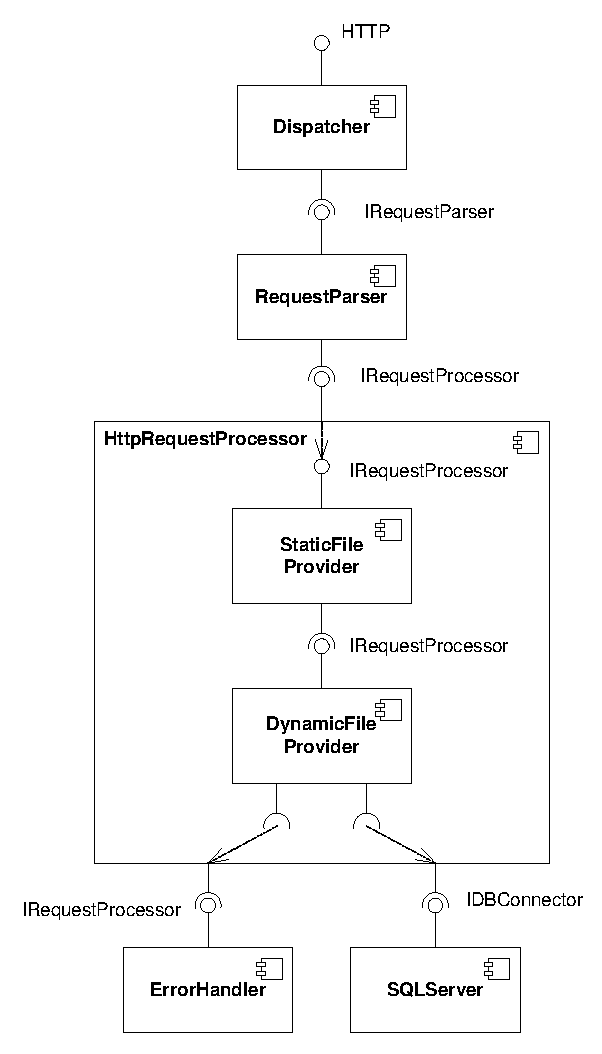
\includegraphics[width=3.3in]{example/WebserverComponents}
\caption{Component architecture of a web server.}
\label{fig:WebserverComponents}
\end{figure}

The main part of the web server is realised by the three components Dispatcher, RequestParser, and HttpRequestProcessor. The Dispatcher listens on a set of incoming connections. For each incoming HTTP request, it spawns a new tread and activates the RequestParser. The parser analyses the request and passes the result to the HttpRequestProcessor. The request processor is organised as a chain of responsability \cite{gamma1995a}. Each of its subcomponents checks whether it can handle the incoming request. If so, it returns the result, otherwise it passes the request to the next component in the chain of responsibility. The ErrorHandler represents the end of the chain and returns an error message if the request could not be handled by any of the components. Additionally, the SQLServer is required to create dynamic HTML pages.


\begin{figure}[htbp]
\centering
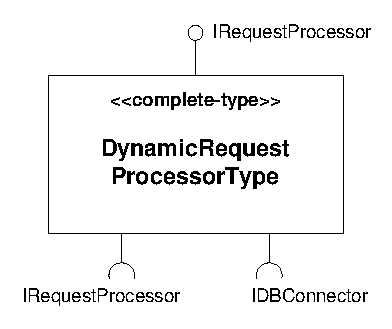
\includegraphics[scale=0.85]{example/DynamicRequestProcessorType}
\caption{Component type for dynamic request processors.}
\label{fig:DynamicRequestProcessorType}
\end{figure}

Looking at the architecture of the web server, we can identify different component types according to the definition in UML 2.0. These types are called \emph{complete-types} in the Palladio Component Meta Model. For example, the components HttpRequestProcessor and DynamicFileProvide provide the IRequestProcessor interface and use the interfaces IDBConnector and IRequestProcessor. The first one is used to create dynamic content of web pages. The second one is required to forward the request to the next component in the chain of responsibility. The corresponding type of both components is shown in figure \ref{fig:DynamicRequestProcessorType}.

\begin{figure}[htbp]
\centering
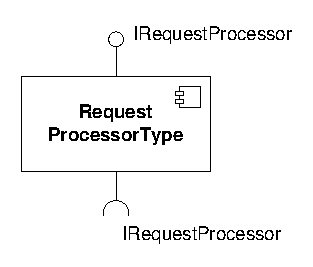
\includegraphics[scale=0.85]{example/RequestProcessorType}
\caption{Another component type used in the web server.}
\label{fig:RequestProcessorType}
\end{figure}

The type of the StaticFileProvider component shown in figure \ref{fig:RequestProcessorType} provides and requires the IRequestProcessor interface only. So, it differs from the DynamicRequestProcessorType, which additionally requires the IDBConnector interface. 

The types shown in figures \ref{fig:DynamicRequestProcessorType} and \ref{fig:RequestProcessorType} are derived from existing components and describe their complete provided and required functionality.
It is obvious that a component conforms to a type if it provides and requires exactly the interfaces specified by the type. However, this is not the case in general. A component is likely to differ from its more general type, but, nevertheless, still be conformant to the type. So, when does a component conform to a type?

A component conforms to a type, if it offers at least the functionality specified by the provided interfaces of the type and uses only the functionality specified by the required interfaces of the type.

For example, a component must offer the IRequestProcessor interface to conform to one of the types in figure \ref{fig:DynamicRequestProcessorType} or \ref{fig:RequestProcessorType}, but it can provide additional interfaces.
Furthermore, a component can only use services that are specified in the required interfaces of the type. The DynamicFileProvider does not conform to the RequestProcessorType, since it uses the IDBConnector interface. Note that a component does not have to use all required interfaces of its type. So, all components that conform to the RequestProcessorType also conform to the DynamicRequestProcessorType, since they do not require the IDBConnectorInterface. 

The definition of conformance corresponds to our view on required and provided interfaces as pre- and postconditions of components (see section \ref{sec:ComponentsInSE}). The precondition can only be weakened. Thus, the component implementation must not use interfaces other than the required interfaces specified by the type. Furthermore, the postcondition can only be strengthened. The component can offer any interfaces, but it must at least provide the ones specified by the type. With this notion of conformance, the type system of components is contravariant.

This understanding of conformance between components and types allows us to define substitutability of components. A component \texttt{A} can be substituted by a component \texttt{B} if \texttt{B} conforms to the type defined by \texttt{A}. The type defined by a component includes all its provided and required interfaces. This is a very pessimistic definition of substitutability, which can be weakened under certain conditions. 

In many cases, we are not only interested in the substitution of complete components including provided and required interfaces, but in a substitution with respect to provided interfaces only. This is the case if the functionality is more important than the requirements of a component or if we compare the functionality offered by different components. Furthermore, it might not be possible to specify all required interfaces of a component in advance. 

\begin{figure}[htbp]
\centering
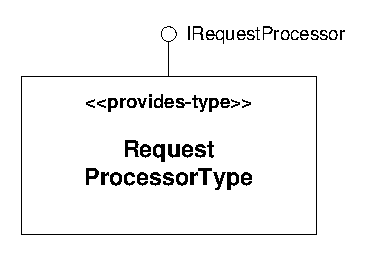
\includegraphics[scale=0.85]{example/ProvidesType}
\caption{provided-type of the RequestProcessorType and DynamicRequestProcessorType.}
\label{fig:ProvidesType}
\end{figure}

Hence, we want to allow conformance with respect to provided interfaces only. Therefore, we introduce a \emph{provided-type} which only considers provided interfaces. The provided-type of the RequestProcessortType and the DynamicRequestProcessorType is shown in figure \ref{fig:ProvidesType}. 
It represents a more abstract view on software components. This is needed, since, during design time, it is often not clear what other components will be needed to implement the desired functionality. Expecting the software architect to decide this would require nearly the same effort as implementing the software component. Thus, the development process of a component should not be fixed to the required interfaces specified by a component type. It rather evolves with the development of the component. Provided and required interfaces are added and removed over time. The system architect specifies a basic set of interfaces that is used by the components to communicate. More interfaces might be added later to implement the functionality of the components.

The stepwise completion of a component specification leads to different interpretations of required interfaces. The change from provided-type to complete-type depends on this interpretation. So far, we identified three different meanings of the specified required interfaces of a type:
\begin{enumerate}
\item	A required interface can be used, but additional interfaces can be added.
\item	Only the listed required interfaces can be used.
\item	A required interface has to be used in a predefined way and certain call sequences have to be executed. 
\end{enumerate}

Required interfaces of the provided-type are not considered explicitly. However, if they are specified, their meaning corresponds to the first case in the list, since, for provided-types, the use of external services is not limited. The second case corresponds to the complete-type. The usage of external services is limited to the required interfaces specified for the component and no further interfaces can be used by the component. The last case expresses additional component requirements. For example, we could specify that all information has to be stored in a database. So, the interface of the database must be called using certain call sequences. However, this is not considered in the Palladio Component Meta Model.

The distinction of provided- and complete-types brings several advantages. By provided-types, we gain a high flexibility during software development. Furthermore, we can define a substitutability focussing on the functionality of a component. On the other hand, complete-types define a strict substitutability. If a component is replaced by another and both conform to the same complete type, we can assure that certain classes of interoperability problem cannot occur. Moreover, complete-types allow a complete specification of the externally visible behaviour of a software component. The co-existence of both concept offers a high flexibility in software architecture design.
